% Created 2017-09-13 Wed 22:59
% Intended LaTeX compiler: pdflatex
\documentclass[11pt]{article}
\usepackage[utf8]{inputenc}
\usepackage[T1]{fontenc}
\usepackage{graphicx}
\usepackage{grffile}
\usepackage{longtable}
\usepackage{wrapfig}
\usepackage{rotating}
\usepackage[normalem]{ulem}
\usepackage{amsmath}
\usepackage{textcomp}
\usepackage{amssymb}
\usepackage{capt-of}
\usepackage{hyperref}
\author{alex}
\date{\today}
\title{}
\hypersetup{
 pdfauthor={alex},
 pdftitle={},
 pdfkeywords={},
 pdfsubject={},
 pdfcreator={Emacs 25.2.1 (Org mode 9.0.10)}, 
 pdflang={English}}
\begin{document}

\tableofcontents

\section{Assignment 1 - Alex Nguyen z3379933 17s2}
\label{sec:orgce30c36}
\subsection{Protocol implementation details}
\label{sec:org19af96c}
\begin{itemize}
\item This implementation is in Python3 (3.6.2) and consists of 4 modules; sender.py, receiver.py, stp\(_{\text{packet.py}}\) and pld\(_{\text{module.py}}\)
\item stp\(_{\text{packet.py}}\) contains the implementation for the segement (header and payload) and features are discussed in the next section. It contains a print\(_{\text{complete}}\)() method which prints properties (used in debugging)
\item pld\(_{\text{module.py}}\) contains the packet loss methods that chooses with a Boolean whether a packet should be dropped (should\(_{\text{transmit}}\)\(_{\text{packet}}\)())
\item sender.py contains a Sender class which implements a blocking singlethreaded event loop that rotates between sending a packet (whilst there are bytes left to send), receiving acks from Receiver in receiver.py. Receiver sits in continual receive\(_{\text{packet}}\) blocking loop and responds accordingly.
\item 3-way STP initiation handshake and 4-way close handshake are implemented in initiate\(_{\text{stp}}\)() and close\(_{\text{stp}}\)() in both Sender and Receiver, which block to progress state until established/closed, after which corresponding flags are toggled. The Fin and Ack Receiver to Sender has been combined into a single 'FA' as per assignment spec example.
\item Single timeout component is implemented by interrupts by a threaded sender.sender\(_{\text{timer}}\)(), which calls sender.retransmit() with the sender.send\(_{\text{base}}\) as an argument to retransmit the right packet when appropriate. Set\(_{\text{timer}}\)() and set\(_{\text{close}}\)\(_{\text{timer}}\)() are methods to modify the timer state.
\item After initiation, Sender's send\(_{\text{packet}}\)(), receive\(_{\text{packet}}\)() and retransmit\(_{\text{packet}}\)() methods handle the main logic, using the combination of a packet\(_{\text{buffer}}\) (to store/track sent packets), next\(_{\text{seq}}\)\(_{\text{num}}\) and send\(_{\text{base}}\) variables according to simpleified TCP sender with fast retransmit
\item Instant acks, no delayed ack and packets respect MWS/MSS respectively - current window size will never exceed the maximum and where possible it will partition into MSS packets
\item For straightforward use of the python socket/pickle libraries, this TCP sender is single-threaded - the event loop follows an order and blocks, though only 1 packet is processed before moving on. To improve, multithreading would  asynchronous event loop would allow for the event loop to match the textbook.
\item Program seems vulnerable to infinite retransmission when the timeout\(_{\text{length}}\) is too low (<3ms) - side-effect of single-threadedness
\end{itemize}
\subsection{STP Header explanation}
\label{sec:org1fd274c}
\begin{itemize}
\item A detailed diagram of your STP header and a quick explanation of all fields (similar to the diagrams that we have used in the lectures to understand TCP/UDP headers).
\end{itemize}
\begin{center}
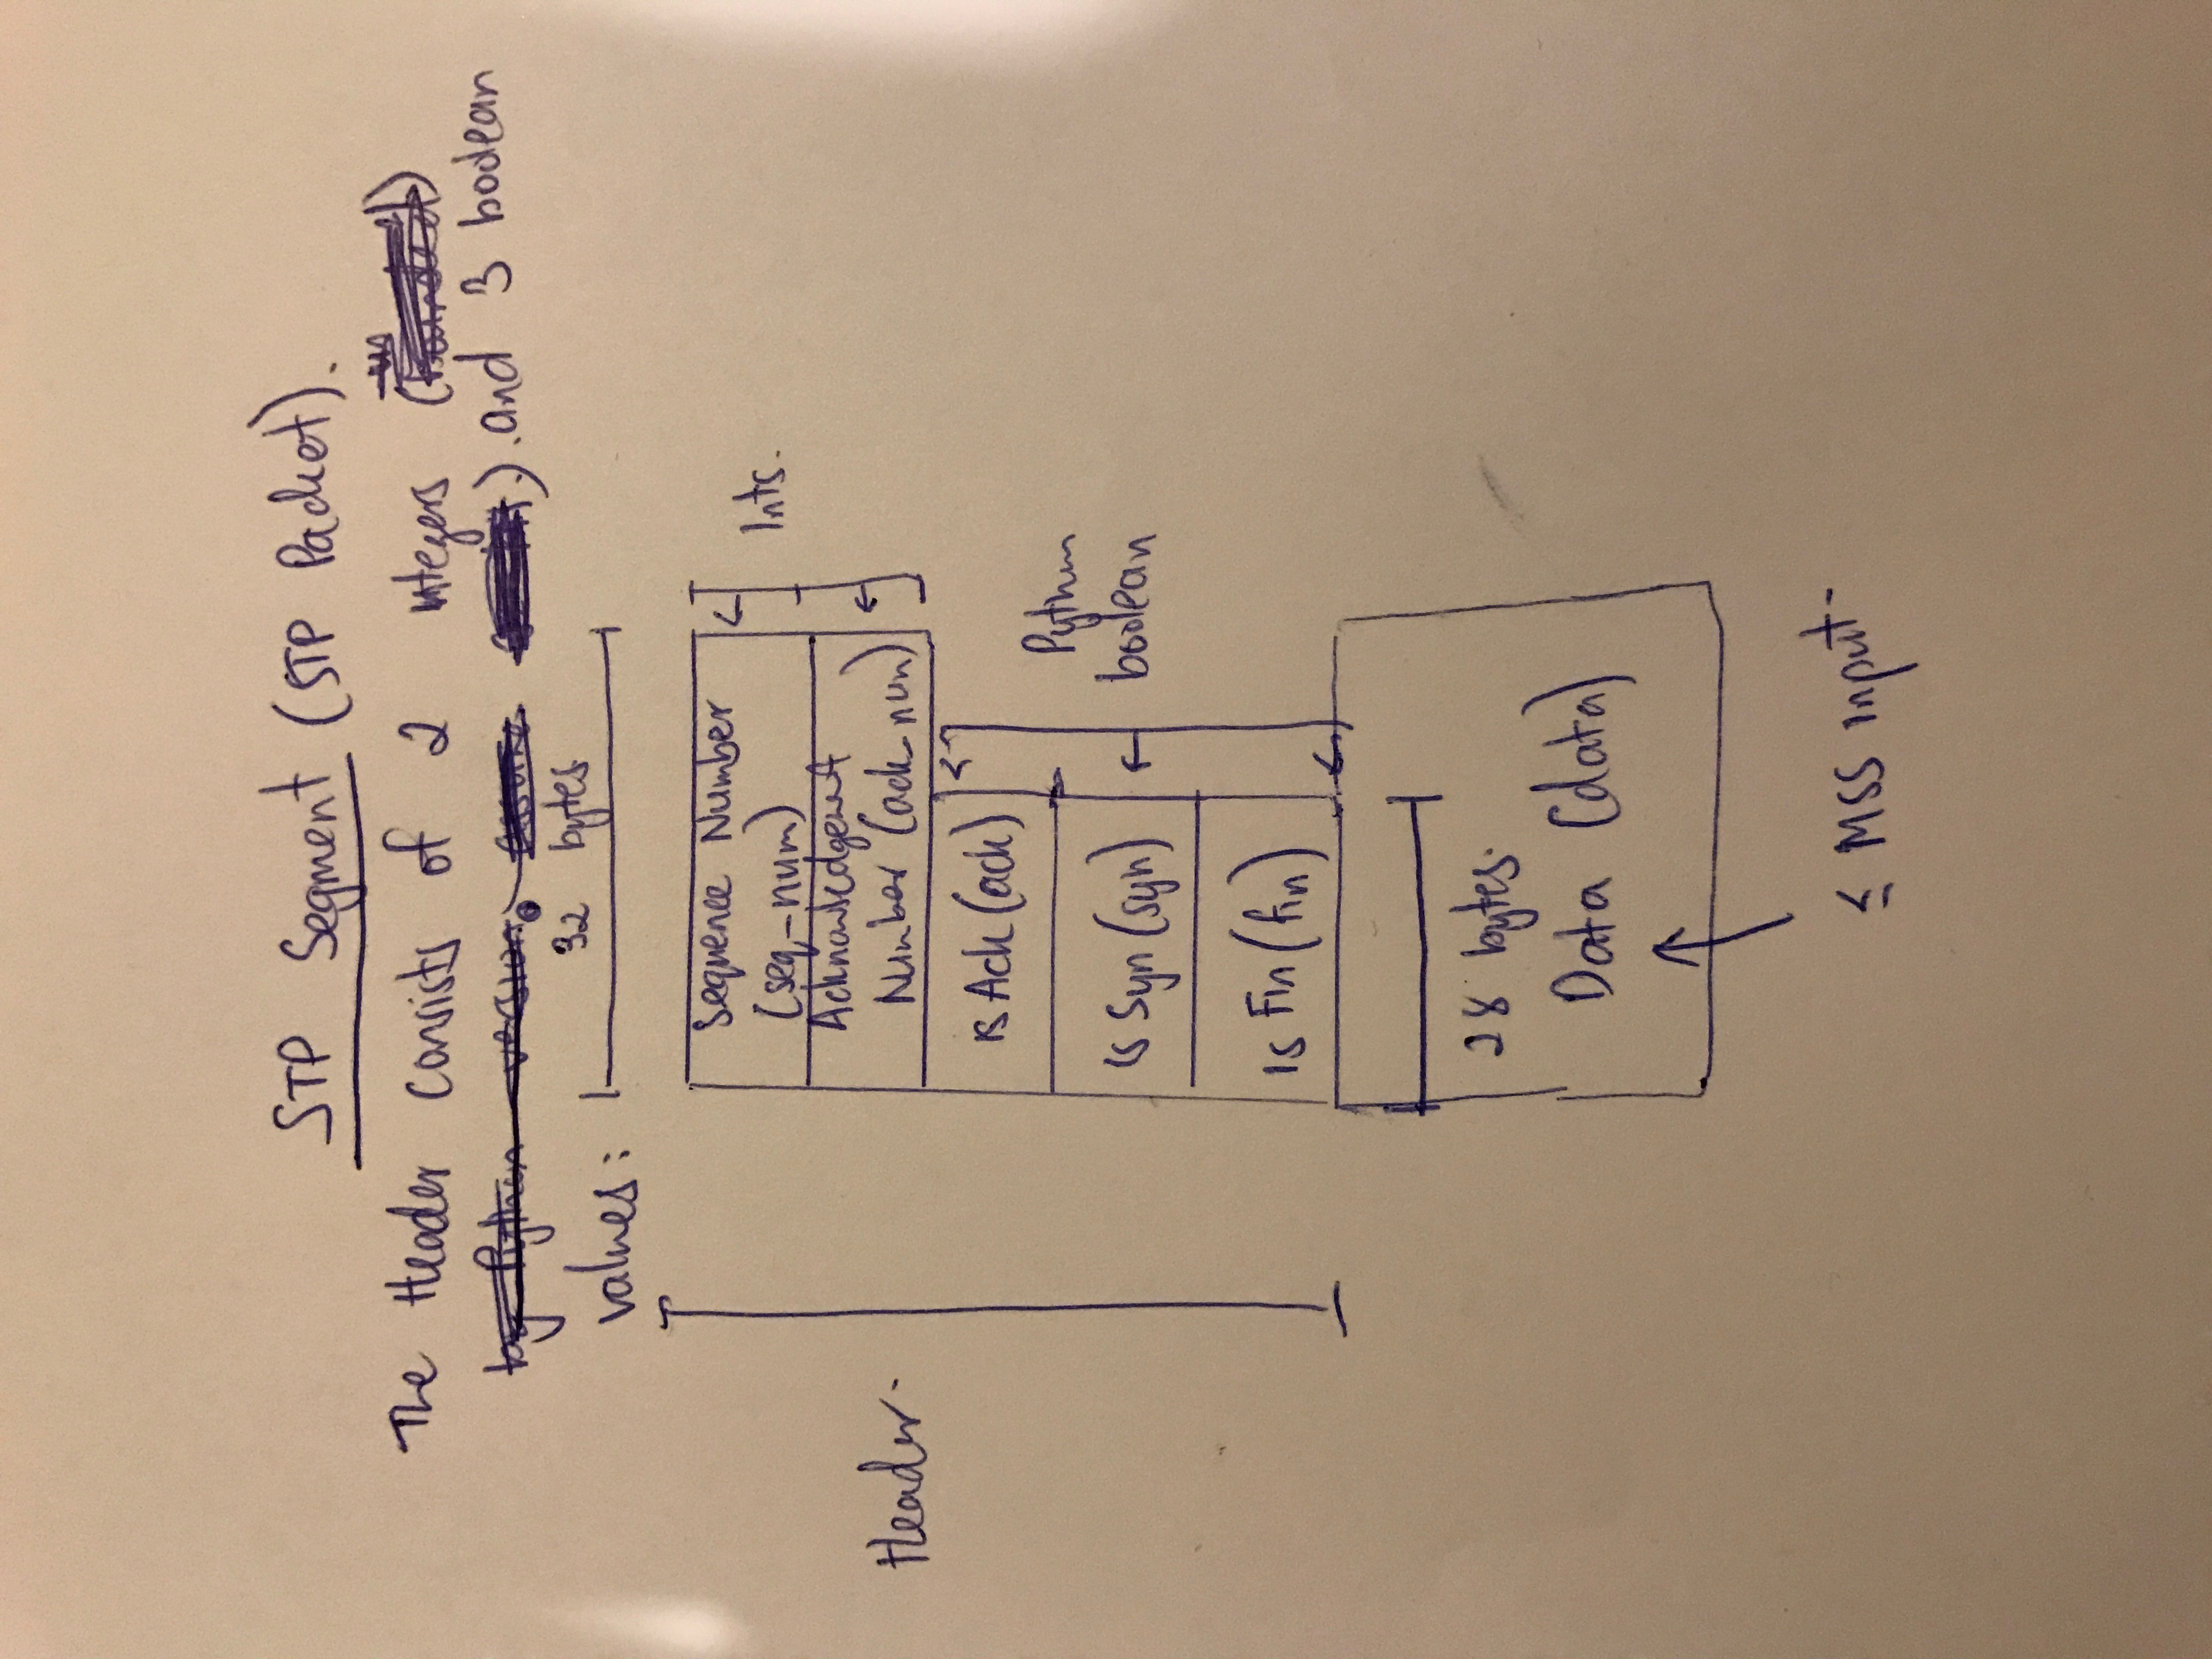
\includegraphics[width=.9\linewidth]{./stp_header.JPG}
\end{center}
 See figure above for a diagram of the STPPacket (stp\(_{\text{packet.py}}\)) used for this assignment.
\begin{itemize}
\item Sequence Number (seq\(_{\text{num}}\)): Sequence number (initially < 1000 for Sender and Receiver) assigned to the packet. This is used for signifying/identifying the first byte of data that the packet contains, and both Sender and Receiver use this number to track the packet they're up to sending and acknowledging, respectively.
\item Acknowledgement Number (ack\(_{\text{num}}\)): This number identifies the last byte accepted by the other party. In ack packets created by Receiver passed to Sender, the ack\(_{\text{num}}\) is a tracking number that increments based on the number of bytes last acknowledged by Receiver.
\item isAck, isSyn, isFin booleans: used to identify Acknowledgement (ack) packets, used in intiating connection (receiver sends response with both Syn and Ack booleans set to True) and closing (receiver sends a packet with Fin and Ack bits set to True to model the 4 way handshake)
\end{itemize}
\subsection{Experiment results}
\label{sec:orge7704f0}
\subsubsection{Part A}
\label{sec:orgb3b1f38}
\begin{itemize}
\item I decided to use 20ms as the timeout value. I experimented with values of 0.5 ms (40x less) and 100ms (5x more) as shown in attached Sender/Receiver\(_{\text{log}}\)\(_{\text{Experiments}}\)\(_{\text{timeout}}\)\(_{\text{fast}}\)/slow.txt files (also see appendix).
\begin{itemize}
\item Longer timeout causes sender to take longer to wait between sending packets and causes deadtime (which can be spent retransmitting to receiver) - In this case, the cost of a timeout is much larger (100ms vs 2ms\textasciitilde{}) of the average time between send and packet receives (timeout\(_{\text{slow.txt}}\) files)
\item Shorter timeout makes use of the time mentioned above, but brings a risk of being caught in a retransmission loop - if the timeout is \textbf{too} short, the sender does not have enough time to receive any packets before a timeout (and hence infinite retransmission) - demonstrated in timeout\(_{\text{fast.txt}}\) files.
\item The trace of Sequence STP packets observed at the receiver ('rcv' packet) at 20ms is shown below with pdrop = 0.1 and 0.3 respectively:
\item See appendix for full trace
\end{itemize}
\end{itemize}
\begin{verbatim}
0.1: 612 613 613 663 713 763 813 863 913 963 1013 1063 1113 1163 1213
1263 1413 1463 1563 1613 1713 1313 1813 1363 1863 1913 1963 1513
2013 2113 1663 2163 1763 2063 2206 2206

0.3: 612 613 613 663 713 763 913 963 1013 1063 1113 1163 1213 1263 813 863 1363
 1463 1613 1663 1713 1763 1313 1313 1413 1963 1513 2013 1563 2063 2113 2163 1813
 1863 1913 2206 2206
\end{verbatim}
\begin{enumerate}
\item Packet loss discussion
\label{sec:org7a0ba7f}
\begin{itemize}
\item In the example above, both sequence number traces start with 612/613/613 and end with 2206 2206 twice as these are used in the intiation and teardown of the STP connection
\item When pdrop is 0.3, packet loss occurs earlier as we can see packet 813 is received much later compared to 0.1 (it is the 7th packet in the latter case, 15th in 0.3). This makes sense as we have increased likelihood of a drop.
\item Increasing pdrop also seems to increase the gap until the delayed packet is received - with 0.1 1313 appears 4 sequence numbers after it is expected, while at 0.3 1313 disappears for much longer - this is side effect of having to wait for more drops to get the packet through.
\item This indicates a higher retrasnmission rate for higher pdrop probabilities values, but appendix shows raw numbers the same duplicates -- possibly due to seeding and shorter length of file
\end{itemize}
\end{enumerate}
\subsubsection{Part B}
\label{sec:orgd504658}
The table below summarises the experiment results:
\begin{center}
\begin{tabular}{lrl}
Time val & STP packets (unique+retransmit) & length of transfer\\
20ms (t) & 56 & 85.5ms\\
80ms (4t) & 56 & 204ms\\
5ms (t/4) & 56 & 58.9ms\\
\end{tabular}
\end{center}

\begin{enumerate}
\item Timeout length Discussion
\label{sec:org6d543f7}
\begin{itemize}
\item Longer timeout resulted in longer overall time to transfer
\item Comments about length from part A apply here; long timeouts force the current form of sender to block on waiting to receive a packet for longer until timeout which interrupts this - make it longer, and overall it will take longer to transfer
\item Each run took the same amount of retransmits/unique per run. This could be because we use the same seed/pdrop for each run; fixing the likelihood of dropping a packet (pld.should\(_{\text{transmit}}\)\(_{\text{packet}}\)()) in the same spot each time.  Also perhaps because this STP sender is not multithreaded - blocking calls are used so a predictable send/receive loop happens each time.
\end{itemize}
\end{enumerate}

\section{Appendix}
\label{sec:org41e84b9}
\subsection{STP Header}
\label{sec:org67cf3eb}
\begin{center}
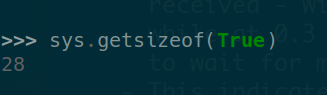
\includegraphics[width=.9\linewidth]{./pythonbool.png}
\end{center}
\subsection{Part A}
\label{sec:orgcfe1811}
\begin{itemize}
\item pdrop = 0.1
\end{itemize}
\begin{verbatim}
rcv 1632.019281387329 S 612 0 0
snd 1632.3606967926025 SA 137 0 613
rcv 1632.7528953552246 A 613 0 138
rcv 1633.1524848937988 D 613 50 138
snd 1633.3940029144287 A 138 0 663
rcv 1634.2799663543701 D 663 50 138
snd 1634.5925331115723 A 138 0 713
rcv 1636.3451480865479 D 713 50 138
snd 1636.5907192230225 A 138 0 763
rcv 1636.7871761322021 D 763 50 138
snd 1636.9709968566895 A 138 0 813
rcv 1638.7922763824463 D 813 50 138
snd 1639.1315460205078 A 138 0 863
rcv 1639.4166946411133 D 863 50 138
snd 1639.6780014038086 A 138 0 913
rcv 1639.9922370910645 D 913 50 138
snd 1640.2370929718018 A 138 0 963
rcv 1642.4074172973633 D 963 50 138
snd 1642.6866054534912 A 138 0 1013
rcv 1643.1975364685059 D 1013 50 138
snd 1643.5065269470215 A 138 0 1063
rcv 1643.751621246338 D 1063 50 138
snd 1644.0362930297852 A 138 0 1113
rcv 1644.7679996490479 D 1113 50 138
snd 1645.0231075286865 A 138 0 1163
rcv 1645.6866264343262 D 1163 50 138
snd 1645.918846130371 A 138 0 1213
rcv 1646.5883255004883 D 1213 50 138
snd 1646.8138694763184 A 138 0 1263
rcv 1647.7339267730713 D 1263 50 138
snd 1647.9730606079102 A 138 0 1313
rcv 1650.270700454712 D 1413 50 138
snd 1650.5649089813232 A 138 0 1313
rcv 1651.1669158935547 D 1463 50 138
snd 1651.3926982879639 A 138 0 1313
rcv 1652.784824371338 D 1563 50 138
snd 1653.0766487121582 A 138 0 1313
rcv 1653.6638736724854 D 1613 50 138
snd 1653.9292335510254 A 138 0 1313
rcv 1655.2174091339111 D 1713 50 138
snd 1655.4720401763916 A 138 0 1313
rcv 1657.2179794311523 D 1313 50 138
snd 1657.4735641479492 A 138 0 1363
rcv 1658.5204601287842 D 1813 50 138
snd 1658.8306427001953 A 138 0 1363
rcv 1659.4476699829102 D 1363 50 138
snd 1659.703016281128 A 138 0 1513
rcv 1660.3660583496094 D 1863 50 138
snd 1660.618543624878 A 138 0 1513
rcv 1661.0779762268066 D 1913 50 138
snd 1661.2935066223145 A 138 0 1513
rcv 1661.6871356964111 D 1963 50 138
snd 1661.935567855835 A 138 0 1513
rcv 1662.8293991088867 D 1513 50 138
snd 1663.064956665039 A 138 0 1663
rcv 1663.8317108154297 D 2013 50 138
snd 1664.0443801879883 A 138 0 1663
rcv 1664.719820022583 D 2113 50 138
snd 1664.924144744873 A 138 0 1663
rcv 1705.6031227111816 D 1663 50 138
snd 1705.9342861175537 A 138 0 1763
rcv 1706.7060470581055 D 2163 43 138
snd 1706.9358825683594 A 138 0 1763
rcv 1707.4129581451416 D 1763 50 138
snd 1707.613468170166 A 138 0 2063
rcv 1728.4271717071533 D 2063 50 138
snd 1728.719711303711 A 138 0 2206
rcv 1729.309320449829 F 2206 0 138
snd 1729.4931411743164 FA 138 0 2206
rcv 1730.008602142334 A 2206 0 138
Amount of (original) Data Received (in bytes): 1593
Number of (original) Data Segments received: 32
Number of Duplicate Segments received: 12
\end{verbatim}
\begin{itemize}
\item pdrop = 0.3
\end{itemize}
\begin{verbatim}
rcv 1611.8731498718262 S 612 0 0
snd 1612.220048904419 SA 137 0 613
rcv 1612.5586032867432 A 613 0 138
rcv 1612.8664016723633 D 613 50 138
snd 1613.1250858306885 A 138 0 663
rcv 1613.75093460083 D 663 50 138
snd 1614.0780448913574 A 138 0 713
rcv 1614.438533782959 D 713 50 138
snd 1614.7871017456055 A 138 0 763
rcv 1615.2734756469727 D 763 50 138
snd 1615.5800819396973 A 138 0 813
rcv 1618.8685894012451 D 913 50 138
snd 1619.1222667694092 A 138 0 813
rcv 1619.3442344665527 D 963 50 138
snd 1619.6284294128418 A 138 0 813
rcv 1619.8501586914062 D 1013 50 138
snd 1620.129108428955 A 138 0 813
rcv 1620.3298568725586 D 1063 50 138
snd 1620.595932006836 A 138 0 813
rcv 1621.4320659637451 D 1113 50 138
snd 1621.6449737548828 A 138 0 813
rcv 1622.4780082702637 D 1163 50 138
snd 1622.743844985962 A 138 0 813
rcv 1623.415470123291 D 1213 50 138
snd 1623.6672401428223 A 138 0 813
rcv 1624.4971752166748 D 1263 50 138
snd 1624.7608661651611 A 138 0 813
rcv 1667.612075805664 D 813 50 138
snd 1667.968511581421 A 138 0 863
rcv 1689.2757415771484 D 863 50 138
snd 1689.5866394042969 A 138 0 1313
rcv 1690.3190612792969 D 1363 50 138
snd 1690.652847290039 A 138 0 1313
rcv 1691.709041595459 D 1463 50 138
snd 1692.2540664672852 A 138 0 1313
rcv 1693.1986808776855 D 1613 50 138
snd 1693.4888362884521 A 138 0 1313
rcv 1694.1442489624023 D 1663 50 138
snd 1694.3538188934326 A 138 0 1313
rcv 1694.6256160736084 D 1713 50 138
snd 1694.8602199554443 A 138 0 1313
rcv 1695.1136589050293 D 1763 50 138
snd 1695.3349113464355 A 138 0 1313
rcv 1696.0875988006592 D 1313 50 138
snd 1696.4771747589111 A 138 0 1413
rcv 1697.2620487213135 D 1313 50 138
snd 1697.561264038086 A 138 0 1413
rcv 1699.5060443878174 D 1413 50 138
snd 1699.8677253723145 A 138 0 1513
rcv 1700.7341384887695 D 1963 50 138
snd 1701.012372970581 A 138 0 1513
rcv 1721.161127090454 D 1513 50 138
snd 1721.4791774749756 A 138 0 1563
rcv 1722.0988273620605 D 2013 50 138
snd 1722.3668098449707 A 138 0 1563
rcv 1742.4774169921875 D 1563 50 138
snd 1742.795705795288 A 138 0 1813
rcv 1743.3545589447021 D 2063 50 138
snd 1743.6230182647705 A 138 0 1813
rcv 1743.866205215454 D 2113 50 138
snd 1744.1179752349854 A 138 0 1813
rcv 1744.3630695343018 D 2163 43 138
snd 1744.6062564849854 A 138 0 1813
rcv 1786.3845825195312 D 1813 50 138
snd 1786.8273258209229 A 138 0 1863
rcv 1807.6775074005127 D 1863 50 138
snd 1807.9912662506104 A 138 0 1913
rcv 1828.8764953613281 D 1913 50 138
snd 1829.2369842529297 A 138 0 2206
rcv 1829.7038078308105 F 2206 0 138
snd 1829.8916816711426 FA 138 0 2206
rcv 1830.3756713867188 A 2206 0 138
Amount of (original) Data Received (in bytes): 1593
Number of (original) Data Segments received: 32
Number of Duplicate Segments received: 20
\end{verbatim}
\subsection{Part B}
\label{sec:org7b82f44}
\begin{itemize}
\item T/4
\end{itemize}
\begin{verbatim}
snd 0.5733966827392578 S 612 0 0
rcv 0.9748935699462891 SA 137 0 613
snd 1.2731552124023438 A 613 0 138
snd 1.7879009246826172 D 613 50 138
snd 2.920866012573242 D 663 50 138
snd 3.501415252685547 D 713 50 138
snd 4.314899444580078 D 763 50 138
snd 4.77290153503418 D 813 50 138
snd 5.400180816650391 D 863 50 138
snd 6.210565567016602 D 913 50 138
snd 8.080244064331055 D 963 50 138
snd 8.62884521484375 D 1013 50 138
snd 9.306192398071289 D 1063 50 138
rcv 9.633302688598633 A 138 0 663
snd 10.367155075073242 D 1113 50 138
rcv 10.792732238769531 A 138 0 713
snd 11.441230773925781 D 1163 50 138
rcv 11.862039566040039 A 138 0 763
snd 12.474536895751953 D 1213 50 138
rcv 12.79449462890625 A 138 0 813
snd 13.40031623840332 D 1263 50 138
rcv 13.714790344238281 A 138 0 863
drop 14.304876327514648 D 1313 50 138
rcv 14.605522155761719 A 138 0 913
drop 15.232563018798828 D 1363 50 138
rcv 15.498161315917969 A 138 0 963
snd 16.073226928710938 D 1413 50 138
rcv 16.318321228027344 A 138 0 1013
snd 16.94798469543457 D 1463 50 138
rcv 17.210721969604492 A 138 0 1063
drop 17.717361450195312 D 1513 50 138
rcv 17.949342727661133 A 138 0 1113
snd 18.644094467163086 D 1563 50 138
rcv 18.917322158813477 A 138 0 1163
snd 19.534587860107422 D 1613 50 138
rcv 19.776582717895508 A 138 0 1213
drop 20.273923873901367 D 1663 50 138
rcv 20.496368408203125 A 138 0 1263
snd 21.02184295654297 D 1713 50 138
rcv 21.24786376953125 A 138 0 1313
drop 21.76499366760254 D 1763 50 138
rcv 21.98481559753418 A 138 0 1313
rcv 22.179841995239258 A 138 0 1313
rcv 22.365093231201172 A 138 0 1313
snd 22.68671989440918 D 1313 50 138
rcv 23.258447647094727 A 138 0 1313
rcv 23.442506790161133 A 138 0 1313
rcv 23.64492416381836 A 138 0 1363
snd 24.308443069458008 D 1813 50 138
rcv 24.54519271850586 A 138 0 1363
snd 24.85799789428711 D 1363 50 138
rcv 25.351524353027344 A 138 0 1513
snd 26.16119384765625 D 1863 50 138
snd 26.661396026611328 D 1913 50 138
snd 27.09054946899414 D 1963 50 138
rcv 27.319669723510742 A 138 0 1513
rcv 27.493953704833984 A 138 0 1513
rcv 27.67038345336914 A 138 0 1513
snd 27.952194213867188 D 1513 50 138
rcv 28.363466262817383 A 138 0 1663
snd 28.93209457397461 D 2013 50 138
drop 29.28638458251953 D 2063 50 138
snd 29.708147048950195 D 2113 50 138
rcv 29.929399490356445 A 138 0 1663
rcv 30.111312866210938 A 138 0 1663
drop 34.88039970397949 D 1663 50 138
snd 40.48514366149902 D 1663 50 138
rcv 40.85421562194824 A 138 0 1763
snd 41.42165184020996 D 2163 50 138
snd 41.92709922790527 D 2213 50 138
rcv 42.14119911193848 A 138 0 1763
snd 42.45805740356445 D 1763 50 138
rcv 42.78230667114258 A 138 0 1763
rcv 42.995452880859375 A 138 0 2063
snd 43.5948371887207 D 2263 50 138
snd 44.06285285949707 D 2313 50 138
snd 44.57998275756836 D 2363 50 138
snd 45.04275321960449 D 2413 50 138
snd 45.47238349914551 D 2463 50 138
snd 45.89557647705078 D 2513 50 138
rcv 46.10323905944824 A 138 0 2063
rcv 46.29969596862793 A 138 0 2063
snd 46.58055305480957 D 2063 50 138
rcv 46.90718650817871 A 138 0 2063
rcv 47.09434509277344 A 138 0 2063
rcv 47.260284423828125 A 138 0 2063
snd 47.53518104553223 D 2063 50 138
rcv 47.873497009277344 A 138 0 2063
rcv 48.062801361083984 A 138 0 2563
snd 48.54154586791992 D 2563 4 138
rcv 48.738956451416016 A 138 0 2563
rcv 48.94280433654785 A 138 0 2567
snd 49.2253303527832 F 2567 0 138
rcv 49.704790115356445 FA 138 0 2567
snd 49.96061325073242 A 2567 0 138
Amount of (original) Data Transferred (in bytes) 1954
Number of  Data Segments Sent (excluding retransmissions) 40
Number of (all) Packets Dropped 7
Number of Retransmitted Segments 16
Number of Duplicate Acknowledgements received 20
\end{verbatim}
\begin{itemize}
\item 4T
\end{itemize}
\begin{verbatim}
 snd 0.5698204040527344 S 612 0 0
rcv 1.0190010070800781 SA 137 0 613
snd 1.4905929565429688 A 613 0 138
snd 2.1202564239501953 D 613 50 138
snd 2.753734588623047 D 663 50 138
snd 3.3617019653320312 D 713 50 138
snd 3.9594173431396484 D 763 50 138
snd 4.74858283996582 D 813 50 138
snd 5.269765853881836 D 863 50 138
snd 5.890846252441406 D 913 50 138
snd 6.387472152709961 D 963 50 138
snd 6.994724273681641 D 1013 50 138
snd 7.740020751953125 D 1063 50 138
rcv 8.003473281860352 A 138 0 663
snd 8.69894027709961 D 1113 50 138
rcv 8.974552154541016 A 138 0 713
snd 9.64808464050293 D 1163 50 138
rcv 9.897708892822266 A 138 0 763
snd 10.554313659667969 D 1213 50 138
rcv 10.81228256225586 A 138 0 813
snd 11.449098587036133 D 1263 50 138
rcv 11.714696884155273 A 138 0 863
drop 12.209653854370117 D 1313 50 138
rcv 12.434959411621094 A 138 0 913
drop 12.920856475830078 D 1363 50 138
rcv 13.145208358764648 A 138 0 963
snd 13.793468475341797 D 1413 50 138
rcv 14.063358306884766 A 138 0 1013
snd 14.91093635559082 D 1463 50 138
rcv 15.129566192626953 A 138 0 1063
drop 15.611648559570312 D 1513 50 138
rcv 15.8233642578125 A 138 0 1113
snd 16.34669303894043 D 1563 50 138
rcv 16.575336456298828 A 138 0 1163
snd 17.141342163085938 D 1613 50 138
rcv 17.37046241760254 A 138 0 1213
drop 17.850637435913086 D 1663 50 138
rcv 18.049001693725586 A 138 0 1263
snd 18.664121627807617 D 1713 50 138
rcv 18.87798309326172 A 138 0 1313
drop 19.396305084228516 D 1763 50 138
rcv 19.617319107055664 A 138 0 1313
rcv 19.807100296020508 A 138 0 1313
rcv 19.983768463134766 A 138 0 1313
snd 20.31397819519043 D 1313 50 138
rcv 20.893573760986328 A 138 0 1313
rcv 21.094083786010742 A 138 0 1313
rcv 21.29340171813965 A 138 0 1363
snd 21.98648452758789 D 1813 50 138
rcv 22.232532501220703 A 138 0 1363
snd 22.562503814697266 D 1363 50 138
rcv 22.93705940246582 A 138 0 1513
snd 23.598194122314453 D 1863 50 138
snd 24.24764633178711 D 1913 50 138
snd 24.787425994873047 D 1963 50 138
rcv 25.007247924804688 A 138 0 1513
rcv 25.178909301757812 A 138 0 1513
rcv 25.357961654663086 A 138 0 1513
snd 25.65455436706543 D 1513 50 138
rcv 25.99477767944336 A 138 0 1663
snd 26.61299705505371 D 2013 50 138
drop 27.385473251342773 D 2063 50 138
snd 27.849912643432617 D 2113 50 138
rcv 28.146028518676758 A 138 0 1663
rcv 28.352737426757812 A 138 0 1663
drop 108.00480842590332 D 1663 50 138
snd 188.63415718078613 D 1663 50 138
rcv 189.1610622406006 A 138 0 1763
snd 190.1538372039795 D 2163 50 138
snd 190.73772430419922 D 2213 50 138
rcv 191.0989284515381 A 138 0 1763
snd 191.4958953857422 D 1763 50 138
rcv 191.94769859313965 A 138 0 1763
rcv 192.19374656677246 A 138 0 2063
snd 192.85988807678223 D 2263 50 138
snd 193.4373378753662 D 2313 50 138
snd 194.0932273864746 D 2363 50 138
snd 194.67782974243164 D 2413 50 138
snd 195.13893127441406 D 2463 50 138
snd 195.6791877746582 D 2513 50 138
rcv 195.91522216796875 A 138 0 2063
rcv 196.11668586730957 A 138 0 2063
snd 196.41852378845215 D 2063 50 138
rcv 196.7756748199463 A 138 0 2063
rcv 196.99406623840332 A 138 0 2063
rcv 197.16286659240723 A 138 0 2063
snd 197.44396209716797 D 2063 50 138
rcv 197.79562950134277 A 138 0 2063
rcv 198.01974296569824 A 138 0 2563
snd 198.4121799468994 D 2563 4 138
rcv 198.63295555114746 A 138 0 2563
rcv 198.83346557617188 A 138 0 2567
snd 199.0988254547119 F 2567 0 138
rcv 199.51558113098145 FA 138 0 2567
snd 199.74637031555176 A 2567 0 138
Amount of (original) Data Transferred (in bytes) 1954
Number of  Data Segments Sent (excluding retransmissions) 40
Number of (all) Packets Dropped 7
Number of Retransmitted Segments 16
Number of Duplicate Acknowledgements received 20

\end{verbatim}
\begin{itemize}
\item T
\end{itemize}
\begin{verbatim}
 snd 4.37164306640625 S 612 0 0
rcv 4.924774169921875 SA 137 0 613
snd 5.340814590454102 A 613 0 138
snd 6.241798400878906 D 613 50 138
snd 7.104158401489258 D 663 50 138
snd 8.481025695800781 D 713 50 138
snd 8.967161178588867 D 763 50 138
snd 9.61613655090332 D 813 50 138
snd 10.227441787719727 D 863 50 138
snd 10.912418365478516 D 913 50 138
snd 11.617660522460938 D 963 50 138
snd 12.12930679321289 D 1013 50 138
snd 12.634515762329102 D 1063 50 138
rcv 13.082504272460938 A 138 0 663
snd 13.783454895019531 D 1113 50 138
rcv 14.084577560424805 A 138 0 713
snd 14.706611633300781 D 1163 50 138
rcv 14.962911605834961 A 138 0 763
snd 15.636205673217773 D 1213 50 138
rcv 16.141176223754883 A 138 0 813
snd 17.101526260375977 D 1263 50 138
rcv 17.317533493041992 A 138 0 863
drop 17.808198928833008 D 1313 50 138
rcv 18.037080764770508 A 138 0 913
drop 18.50104331970215 D 1363 50 138
rcv 18.72539520263672 A 138 0 963
snd 19.309520721435547 D 1413 50 138
rcv 19.540071487426758 A 138 0 1013
snd 20.51091194152832 D 1463 50 138
rcv 20.757436752319336 A 138 0 1063
drop 21.31795883178711 D 1513 50 138
rcv 23.433208465576172 A 138 0 1113
snd 26.14140510559082 D 1563 50 138
rcv 26.426076889038086 A 138 0 1163
snd 27.146339416503906 D 1613 50 138
rcv 27.781009674072266 A 138 0 1213
drop 28.36298942565918 D 1663 50 138
rcv 28.644323348999023 A 138 0 1263
snd 31.01491928100586 D 1713 50 138
rcv 31.249523162841797 A 138 0 1313
drop 31.679153442382812 D 1763 50 138
rcv 31.881332397460938 A 138 0 1313
rcv 32.0587158203125 A 138 0 1313
rcv 32.228708267211914 A 138 0 1313
snd 32.590627670288086 D 1313 50 138
rcv 33.004045486450195 A 138 0 1313
rcv 33.19239616394043 A 138 0 1313
rcv 33.377647399902344 A 138 0 1363
snd 33.95581245422363 D 1813 50 138
rcv 34.210205078125 A 138 0 1363
snd 34.55376625061035 D 1363 50 138
rcv 34.90114212036133 A 138 0 1513
snd 35.56108474731445 D 1863 50 138
snd 36.07988357543945 D 1913 50 138
snd 36.61918640136719 D 1963 50 138
rcv 36.86237335205078 A 138 0 1513
rcv 37.04977035522461 A 138 0 1513
rcv 37.22500801086426 A 138 0 1513
snd 37.517547607421875 D 1513 50 138
rcv 37.91642189025879 A 138 0 1663
snd 38.52248191833496 D 2013 50 138
drop 38.89322280883789 D 2063 50 138
snd 39.33262825012207 D 2113 50 138
rcv 39.582252502441406 A 138 0 1663
rcv 39.7794246673584 A 138 0 1663
drop 59.49115753173828 D 1663 50 138
snd 80.12056350708008 D 1663 50 138
rcv 80.45315742492676 A 138 0 1763
snd 81.14099502563477 D 2163 50 138
snd 81.70628547668457 D 2213 50 138
rcv 81.95328712463379 A 138 0 1763
snd 82.26346969604492 D 1763 50 138
rcv 82.61752128601074 A 138 0 1763
rcv 82.83638954162598 A 138 0 2063
snd 83.37140083312988 D 2263 50 138
snd 83.86421203613281 D 2313 50 138
snd 84.37275886535645 D 2363 50 138
snd 84.87653732299805 D 2413 50 138
snd 85.3414535522461 D 2463 50 138
snd 85.86525917053223 D 2513 50 138
rcv 86.1060619354248 A 138 0 2063
rcv 86.30061149597168 A 138 0 2063
snd 86.58051490783691 D 2063 50 138
rcv 86.94291114807129 A 138 0 2063
rcv 87.1577262878418 A 138 0 2063
rcv 87.32175827026367 A 138 0 2063
snd 87.59641647338867 D 2063 50 138
rcv 87.93282508850098 A 138 0 2063
rcv 88.1497859954834 A 138 0 2563
snd 88.5477066040039 D 2563 4 138
rcv 88.77944946289062 A 138 0 2563
rcv 88.99140357971191 A 138 0 2567
snd 89.24484252929688 F 2567 0 138
rcv 89.65659141540527 FA 138 0 2567
snd 89.88404273986816 A 2567 0 138
Amount of (original) Data Transferred (in bytes) 1954
Number of  Data Segments Sent (excluding retransmissions) 40
Number of (all) Packets Dropped 7
Number of Retransmitted Segments 16
Number of Duplicate Acknowledgements received 20

\end{verbatim}
\end{document}
